\documentclass[english,german]{beamer}
\usetheme{naked}

\usepackage{listings}

\usepackage[utf8]{inputenc}
\usepackage[T1]{fontenc}

% (picture proportions: 63 : 20, *.eps format if you use latex+dvips+ps2pdf,
% *.jpg/*.png/*.pdf if you use pdflatex)

\title{Invasive Data Flow Analysis}
\date{\today}
\institute{Fakultät für Informatik -- IPD Snelting}
\author{Andreas Zwinkau}

\begin{document}
%\selectlanguage{english}

\titlepage

\section{X10 Example}

\begin{frame}
\begin{center}
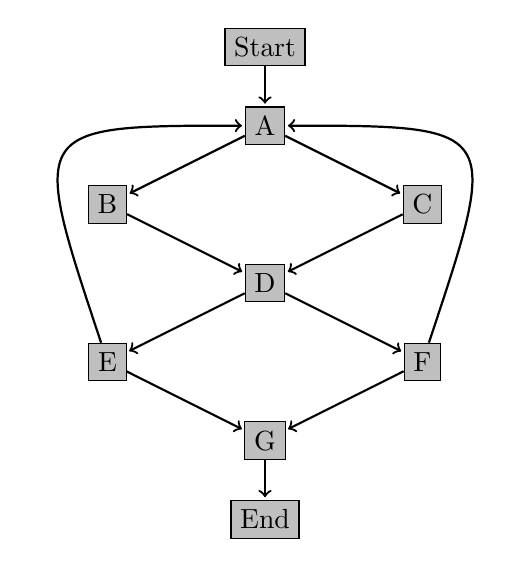
\begin{tikzpicture}
\tikzstyle{dep}= [->,thick,shorten >=1pt]
\tikzstyle{bb}= [rectangle,draw,fill=lightgray]

\path
	( 0, 0) node[bb] (start) {Start}
	( 0,-1) node[bb] (a) {A}
	(-2,-2) node[bb] (b) {B}
	( 2,-2) node[bb] (c) {C}
	( 0,-3) node[bb] (d) {D}
	(-2,-4) node[bb] (e) {E}
	( 2,-4) node[bb] (f) {F}
	( 0,-5) node[bb] (g) {G}
	( 0,-6) node[bb] (end) {End}
;
\draw[dep] (start) -> (a);
\draw[dep] (a) -> (b);
\draw[dep] (a) -> (c);
\draw[dep] (b) -> (d);
\draw[dep] (c) -> (d);
\draw[dep] (d) -> (e);
\draw[dep] (d) -> (f);
\draw[dep] (e) .. controls (-3,-1) .. (a);
\draw[dep] (f) .. controls ( 3,-1) .. (a);
\draw[dep] (e) -> (g);
\draw[dep] (f) -> (g);
\draw[dep] (g) -> (end);
\end{tikzpicture}
\end{center}
\end{frame}

\begin{frame}
$out$(B) = $f_B$($in$(B)) %= ($in$(B) - $kill$(B)) $\cup$ $gen$(B)
\vfill
\begin{center}
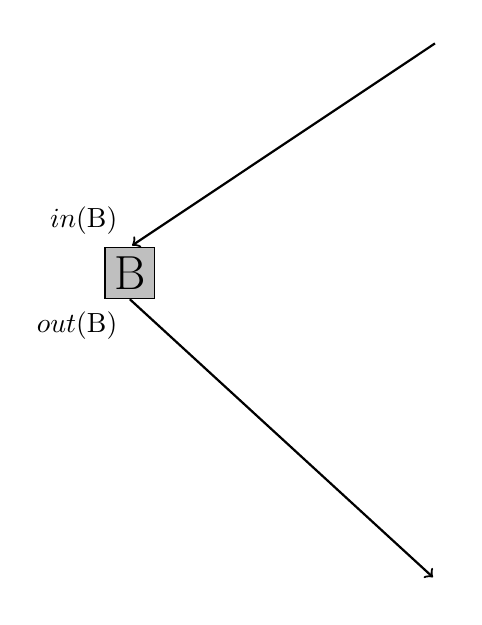
\begin{tikzpicture}
\tikzstyle{dep}= [->,thick,shorten >=1pt]
\tikzstyle{bb}= [rectangle,draw,fill=lightgray]

\path
	( 0,-1) node[] (a) {}
	(-4,-4) node[bb] (b) {\LARGE B}
	( 0,-8) node[] (d) {}
;
\draw[dep] (a) -> (b.north);
\draw[dep] (b.south) -> (d);
\node[above left=1pt] at (b.north) {$in$(B)};
\node[below left=1pt] at (b.south) {$out$(B)};
\end{tikzpicture} \\
\end{center}
\end{frame}

\begin{frame}
$in$(D) = $out$(B) $\sqcup$ $out$(C)
\vfill
\begin{center}
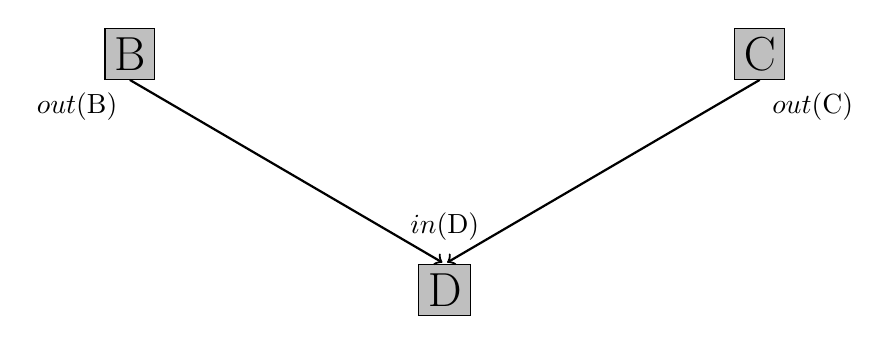
\begin{tikzpicture}
\tikzstyle{dep}= [->,thick,shorten >=1pt]
\tikzstyle{bb}= [rectangle,draw,fill=lightgray]

\path
	(-4, 0) node[bb] (b) {\LARGE B}
	( 4, 0) node[bb] (c) {\LARGE C}
	( 0,-3) node[bb] (d) {\LARGE D}
;
\draw[dep] (b.south) -> (d.north);
\draw[dep] (c.south) -> (d.north);
\node[above =5pt] at (d.north) {$in$(D)};
\node[below left=1pt] at (b.south) {$out$(B)};
\node[below right=1pt] at (c.south) {$out$(C)};
\end{tikzpicture} \\
\end{center}
\end{frame}

\begin{frame}
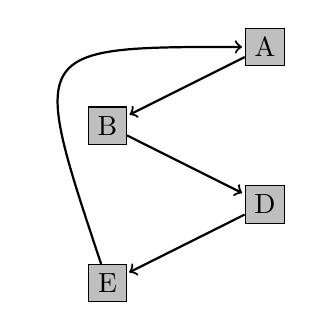
\begin{tikzpicture}
\tikzstyle{dep}= [->,thick,shorten >=1pt]
\tikzstyle{bb}= [rectangle,draw,fill=lightgray]
\path
	( 0,-1) node[bb] (a) {A}
	(-2,-2) node[bb] (b) {B}
	( 0,-3) node[bb] (d) {D}
	(-2,-4) node[bb] (e) {E}
;
\draw[dep] (a) -> (b);
\draw[dep] (b) -> (d);
\draw[dep] (d) -> (e);
\draw[dep] (e) .. controls (-3,-1) .. (a);
\end{tikzpicture} \\
$out$(A) = $f_A$($out$(Start) $\sqcup$ $out$(E) $\sqcup$ $out$(F)) \\
$out$(B) = $f_B$($out$(A)) \\
$out$(D) = $f_D$($out$(B) $\sqcup$ $out$(C)) \\
$out$(E) = $f_E$($out$(D)) \\
\dots \\
\vfill
{\bf\large $\Rightarrow$ Fixpunktiteration}
\end{frame}

\begin{frame}\tt
def analyse( \\
\hspace{0.2cm}	graph:GlobalRef[Array[Node](1)], \\
\hspace{0.2cm}	nodeid:int) \{
\vfill
val current:Node = \\
\hspace{0.2cm}	at (graph.home) (graph()(nodeid)); \\
/* ... expensive analysis here ...  */ \\
if (!changed) return; \\
\vfill
\end{frame}

\begin{frame}\tt
val succ\_count = succs.size(); \\
val claim = Invasion.invade( \\
\hspace{0.2cm}	(place:Place) => (getLoad(place) < 1.0), \\
\hspace{0.2cm}	Invasion.count(succ\_count)); \\
\vfill
claim.infect((p:Point) => \{ \\
\hspace{0.2cm}	analyse(graph, succs(p)); \\
\}); \\
\vfill
claim.retreat(); \\
\}
\end{frame}

\begin{frame}
Thanks
\end{frame}

\end{document}

